\documentclass[english, aspectratio=169]{beamer}
% english is for the language used in standard texts (figures, tables etc)
% aspectratio of 16:9 or set it for more old school to 4:3 (without the ':')

% ---------------------------------------------------------------------------- %
% Load base preamble
% ---------------------------------------------------------------------------- %
\usepackage{import}
\subimport{../preamble/}{beamer.tex}

% ---------------------------------------------------------------------------- %
% Local settings
% ---------------------------------------------------------------------------- %
\newcommand{\B}[0]{\ensuremath{\mathbb{B}}}

\newcommand{\sort}[0]{\text{sort}}

\newcommand{\triple}[3]{\ensuremath{(#1, #2, #3)}}
\renewcommand{\arc}[3]{\ensuremath{#1 \xrightarrow{_{#2}} #3}}

\tikzstyle{plot_adiar}=[color=black, mark=o, mark size=1pt, line width=0.7pt]
\tikzstyle{plot_buddy}=[color=red, mark=o, mark size=1pt, line width=0.7pt]
\tikzstyle{plot_cudd}=[color=blue, mark=diamond, mark size=1pt, line width=0.7pt]
\tikzstyle{plot_sylvan}=[color=purple, mark=square, mark size=1pt, line width=0.7pt]

% Horizontal legends: https://tex.stackexchange.com/a/101578
% argument #1: any options
\makeatletter
\newenvironment{customlegend}[1][]{%
    \begingroup
    % inits/clears the lists (which might be populated from previous
    % axes):
    \pgfplots@init@cleared@structures
    \pgfplotsset{#1}%
}{%
    % draws the legend:
    \pgfplots@createlegend
    \endgroup
}%

% makes \addlegendimage available (typically only available within an
% axis environment):
\def\addlegendimage{\pgfplots@addlegendimage}
\makeatother

% ------------------------------------------------------------------------------
% TITLEPAGE
% ------------------------------------------------------------------------------
\title{
  I/O-efficient Symbolic Model Checking
}
%\subtitle{Decision Diagrams in External Memory}

\author{\textbf{Steffan Christ S\o lvsten}, Jaco van de Pol}

\institute{
\includegraphics[width=0.2\linewidth]{../external/aulogo_uk_var2_black.eps}}

\date{$31^{\text{st}}$ of August, 2022}

\begin{document}

\titleframe

\begin{frame}[plain,noframenumbering]{} % \blankframe until reveal
  \pause

  \begin{center}
    \vspace{8pt}

    {\Huge \textbf{Adiar}}

    \vspace{12pt}

    \textcolor{gray}{\small
      \href{http://github.com/ssoelvsten/adiar}{github.com/ssoelvsten/adiar}
    }
  \end{center}
\end{frame}

% ------------------------------------------------------------------------------
% PRELIMINARIES
% ------------------------------------------------------------------------------

\begin{frame}[plain,noframenumbering]{} % \blankframe until reveal
  \begin{figure}
    \centering

    \only<1>{
      \setvalue{timeline_c0 = gray}
      \setvalue{timeline_c1 = gray}
      \setvalue{timeline_c2 = gray}
    }
    \only<2>{
      \setvalue{timeline_c0 = orange}
      \setvalue{timeline_c1 = gray}
      \setvalue{timeline_c2 = gray}
    }

    \begin{tikzpicture}
      % Primary line
\draw[thick] (0,0) -- (4,0);
\draw[thick] (4.1,0.2) -- (3.9,-0.2);

\draw[-latex, thick] (4.3,0) -- (12,0);
\draw[thick] (4.4,0.2) -- (4.2,-0.2);

% 1985
\draw (0.1,-0.1) -- ++(0,0.2);
\node at (0.1,-0.3) (y1985) {\tiny $1985$} ;

\draw[dashed, color=\getvalue{timeline_c0}] (0.6,0) -- ++(0,0.8);
\node[color=\getvalue{timeline_c0}, align=left] at (1.4,1.3)
(bryant_1986)
{\footnotesize Bryant (1986)\\Binary Decision Diagram (BDD)};

\draw[dashed, color=\getvalue{timeline_c0}] (0.9,-0) -- ++(0,-0.7);
\node[color=\getvalue{timeline_c0}, align=left] at (0.9,-1.3)
(aggarval_1987)
{\footnotesize Aggarwal \& Vitter (1987)\\I/O-model};

% 1990
\draw (1.8,-0.1) -- ++(0,0.2);
\node at (1.8,-0.3) (y1990) {\tiny $1990$};

% 1995
\draw (3.4,-0.1) -- ++(0,0.2);
\node at (3.4,-0.3) (y1995) {\tiny $1995$};

\draw[dashed, color=\getvalue{timeline_c0}] (3.75,0) -- ++(0,-1.5);
\node[color=\getvalue{timeline_c0}, align=left] at (3.7,-2.1)
(arge_1995)
{\footnotesize Arge (1995)\\BDD + I/O-model};

\draw[dashed, color=\getvalue{timeline_c1}] (4.8,0) -- ++(0,0.8);
\node[color=\getvalue{timeline_c1}, align=left] at (5,1.3)
(v1_0)
{\footnotesize Adiar v1.0\\BDD};

% 2022
\draw (5.8,-0.1) -- ++(0,0.2);
\node at (5.8,-0.3) (y2023)  {\tiny $2022$};

\draw[dashed, color=\getvalue{timeline_c1}] (6.2,0) -- ++(0,-0.8);
\node[color=\getvalue{timeline_c1}, align=left] at (6.2,-1.3)
(v1_1)
{\footnotesize Adiar v1.1\\ZDD};

\draw[dashed, color=\getvalue{timeline_c1}] (7,0) -- ++(0,0.8);
\node[color=\getvalue{timeline_c1}, align=left] at (7.5,1.25)
(v1_2)
{\footnotesize Adiar v1.2\\Internal Memory};

% 2023
\draw (8.5,-0.1) -- ++(0,0.2);
\node at (8.5,-0.3) {\tiny $2023$} (y2023);

\draw[dashed, color=\getvalue{timeline_c2}] (9,0) -- ++(0,-0.8);
\node[color=\getvalue{timeline_c2}, align=left] at (10.3,-1.65)
(v2_0)
{\footnotesize Adiar v2.0\\Multi-variable Quantification\\(Multi-recursion)};

\draw[dashed, color=\getvalue{timeline_c2}] (10.5,0) -- ++(0,0.8);
\node[color=\getvalue{timeline_c2}, align=left] at (10.9,1.25)
(v2_1)
{\footnotesize Adiar v2.1\\Variable Reordering};

% 2024
\draw (11.4,-0.1) -- ++(0,0.2);
\node at (11.4,-0.3) (y2024) {\tiny $2024$};

    \end{tikzpicture}
  \end{figure}
\end{frame}

\blankframe

\begin{frame}
  \frametitle{Aggarwal and Vitter '87 : I/O-model}

  \begin{figure}
    \centering

    \begin{tikzpicture}
  % ALU
  \node[
  draw,
  trapezium,
  shape border rotate=180,
  text width=1cm,
  align=center,
  ] at (0.03,0) (cpu) {CPU};

  % Main memory
  \begin{scope}
    \clip(-1.13,1) rectangle (1.19,1.4);
    \filldraw[
    color=black!60!white,
    fill=black!5!white,
    pattern=vertical lines,
    pattern color=black!30!white
    ] (-9,1.25) rectangle ++(18,0.5)
    ;
  \end{scope}

  \node[
  draw,
  rectangle,
  text width=2.08cm,
  align=center,
  ] at (0.03,1.5) (m) {$M$};

  % Disk
  \begin{scope}
    \clip(-6,2.5) rectangle (6,2.9);
    \filldraw[
    color=black!60!white,
    fill=black!5!white,
    pattern=vertical lines,
    pattern color=black!30!white
    ] (-9,2.75) rectangle ++(18,0.5)
    ;
  \end{scope}

  \node[
  draw,
  rectangle,
  text width=5.04cm,
  align=center,
  ] at (0.03,3) (n) {$N$};

  \path[->]
  (cpu) edge[bend left=40] (m)
  (m) edge[bend left=40] (cpu)

  (n) edge[bend left=40] (m)
  (m) edge[bend left=40] (n)
  ;

  \node at (0.02,2.24) {\textcolor{gray}{$B$}};
\end{tikzpicture}


    \caption{The I/O-model by Aggarwal and Vitter '87}
  \end{figure}
\end{frame}

\begin{frame}
  \frametitle{Aggarwal and Vitter '87 : I/O-model}

  For any realistic values of $N$, $M$, and $B$ we have that

  \begin{equation*}
    N/B \quad < \quad \sort(N) \triangleq N/B \cdot \log_{M/B} N/B \quad \ll \quad N
    \enspace ,
  \end{equation*}

  \begin{theorem}[Aggarwal and Vitter '87]
    $N$ elements can be sorted in $\Theta(\sort(N))$ I/Os.
  \end{theorem}
  \begin{theorem}[Arge '95]
    $N$ elements can be inserted in and extracted from a Priority Queue in
    $\Theta(\sort(N))$ I/Os.
  \end{theorem}
\end{frame}

\blankframe

\begin{frame}
  \frametitle{Bryant '86 : Binary Decision Diagram}

  \begin{figure}
    \centering

    \begin{subfigure}{0.49\linewidth}
      \centering

      \begin{tikzpicture}[scale=0.8, every node/.style={transform shape}]
          % nodes
  \node[shape = circle, draw = black]
  (0) {$x_0$};

  \node[shape = circle, draw = black, below right= .4cm and .5cm of 0]
  (1) {$x_1$};

  \node[shape = circle, draw = black, below left=.4cm and .5cm of 1]
  (2) {$x_2$};

  \node[shape = circle, draw = black, below left=.4cm and .5cm of 2]
  (31) {$x_3$};
  \node[shape = circle, draw = black, below right=.4cm and .5cm of 2]
  (32) {$x_3$};

  % leafs
  \node[shape = rectangle, draw = black, below=.4cm of 31]
  (sink_T) {$\top$};

  \node[shape = rectangle, draw = black, below=.4cm of 32]
  (sink_F) {$\bot$};

  % arcs
  \draw[->, dashed]
    (0)  edge (2)
    (1)  edge (2)
    (2)  edge (31)
    (31) edge (sink_T)
    (32) edge (sink_F)
  ;

  \draw[->]
    (0)  edge (1)
    (1)  edge (32)
    (2)  edge (32)
    (31) edge (sink_F)
    (32) edge (sink_T)
  ;
      \end{tikzpicture}

      \caption{$(x_0 \wedge x_1 \wedge x_3) \vee (x_2 \oplus x_3)$}
    \end{subfigure}
    \begin{subfigure}{0.49\linewidth}
      \centering

      \begin{tikzpicture}[scale=0.8, every node/.style={transform shape}]
          % nodes
  \node[shape = circle, draw = black]
  (0) {$x_0$};

  \node[shape = circle, draw = black, below left=1.4cm and .5cm of 0]
  (21) {$x_2$};

  \node[shape = circle, draw = black, below right=1.4cm and .5cm of 0]
  (22) {$x_2$};

  \node[shape = circle, draw = black, below right=0.4cm and .5cm of 21]
  (3) {$x_3$};

  % leafs
  \node[shape = rectangle, draw = black, below right=.4cm and .5cm of 3]
  (sink_F) {$\bot$};

  \node[shape = rectangle, draw = black, below left=.4cm and .5cm of 3]
  (sink_T) {$\top$};

  % arcs
  \draw[->, dashed]
    (0)  edge (21)
    (21) edge (sink_T)
    (22) edge (3)
    (3)  edge (sink_T)
  ;

  \draw[->]
    (0)  edge (22)
    (21) edge (3)
    (22) edge (sink_F)
    (3)  edge (sink_F)
  ;
      \end{tikzpicture}

      \caption{$\neg (x_0 \ ?\ x_2 \vee x_3 \ :\ x_2 \wedge x_3)$}
    \end{subfigure}

    \caption{Examples of (Reduced Ordered) Binary Decision Diagrams.}
  \end{figure}
\end{frame}

\begin{frame}
  \frametitle{Bryant '86 : Binary Decision Diagram}

  \begin{theorem}
    For a fixed variable order, if one exhaustively applies the two rules below,
    then one obtains the Reduced OBDD, which is a unique canonical form of the
    function.
  \end{theorem}

  \begin{figure}
    \centering

    \begin{subfigure}[b]{0.40\linewidth}
      \centering

      \begin{tikzpicture}[scale=0.9, every node/.style={transform shape}]
        \node[shape = circle, black, draw = black] (i) {$x_i$};
\node[shape = circle, draw = black, below=of i] (child) {};
\node[shape = circle, draw = black, above=of i] (parent) {};

% implication
\node[shape = circle, black,right=0.5cm of i] {$\implies$};

% after
\node[shape = circle, draw = black, right=2.5cm of child] (childafter) {};
\node[shape = circle, draw = black, right=2.5cm of parent] (parentafter) {};

\draw[->, dashed] (i) edge[bend right] (child);
\draw[->]
(i) edge[bend left] (child)
(parent) edge (i)
(parentafter) edge (childafter)
;

      \end{tikzpicture}

      \vspace{10pt}
      {\small {\bf (1)} Remove redundant nodes}
    \end{subfigure}
    \begin{subfigure}[b]{0.59\linewidth}
      \centering

      \begin{tikzpicture}[scale=0.9, every node/.style={transform shape}]
        \node[shape = circle, black, draw = black] (i1) {$x_i$};
\node[shape = circle, black, draw = black, right=of i1] (i2) {$x_i$};

\node[shape = circle, draw = black, below=of i1] (child1) {};
\node[shape = circle, draw = black, below=of i2] (child2) {};

\node[shape = circle, draw = black, above=of i1] (parent1) {};
\node[shape = circle, draw = black, above=of i2] (parent2) {};

% implication
\node[shape = circle, black,right=0.5cm of i2] {$\implies$};

% after
\node[shape = circle, draw = black, right=4cm of child1] (c1a) {};
\node[shape = circle, draw = black, right=4cm of child2] (c2a) {};

\node[shape = circle, black, draw = black, right=2.7cm of i2] (ia) {$x_i$};

\node[shape = circle, draw = black, right=4cm of parent1] (p1a) {};
\node[shape = circle, draw = black, right=4cm of parent2] (p2a) {};


\draw[->, dashed]
(i1) edge (child1)
(i2) edge (child1)
(ia) edge (c1a)
;
\draw[->]
(i1) edge (child2)
(i2) edge (child2)
(parent1) edge (i1)
(parent2) edge (i2)
(p1a) edge (ia)
(p2a) edge (ia)
(ia) edge (c2a)
;

      \end{tikzpicture}

      \vspace{10pt}
      {\small {\bf (2)} Merge duplicate nodes}
    \end{subfigure}

  \end{figure}

\end{frame}

\blankframe

\begin{frame}
  \frametitle{Arge '95 : BDD + I/O-model}

  \begin{figure}
    \centering

    \begin{tikzpicture}
      \begin{axis}[%
        width=0.69\linewidth, height=0.42\linewidth,
        every tick label/.append style={font=\scriptsize},
        % x-axis
        xlabel={Table Size (GiB)},
        xmajorgrids=true,
        xmin=3.5,
        xmax=10.5,
        xtick={4, ..., 10},
        % y-axis
        ylabel={time (seconds)},
        yminorgrids=false,
        ymajorgrids=true,
        grid style={dashed,black!20},
        ]

        \draw [white, pattern=north west lines, pattern color=black!30!white]
        (axis cs: 8, 0) rectangle (axis cs: 10, 3000);

        \addplot[thick, samples=1, smooth, black, name path=barrier]
        coordinates {(8,0)(8,3000)};

        \node[black] at (axis cs: 7.6, 2800){\tiny{RAM}};
        \node[black] at (axis cs: 8.4, 2800){\tiny{Swap}};

        \addplot [style=plot_buddy]
        table {./data/cache_buddy_swap.tex};
      \end{axis}
    \end{tikzpicture}

    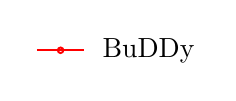
\begin{tikzpicture}
      \begin{customlegend}[
        legend columns=-1,
        legend style={draw=none,column sep=1ex},
        legend entries={BuDDy}
        ]
        \addlegendimage{style=plot_buddy}
      \end{customlegend}
    \end{tikzpicture}

    \caption{Running time for solving a problem that does not need more than $3$ GiB.}
  \end{figure}
\end{frame}

\blankframe

% ------------------------------------------------------------------------------
% CURRENT WORK
% ------------------------------------------------------------------------------
\begin{frame}[plain,noframenumbering]{} % \blankframe until reveal
  \begin{figure}
    \centering

    \setvalue{timeline_c0 = gray}
    \setvalue{timeline_c1 = orange}
    \setvalue{timeline_c2 = gray}

    \begin{tikzpicture}
      % Primary line
\draw[thick] (0,0) -- (4,0);
\draw[thick] (4.1,0.2) -- (3.9,-0.2);

\draw[-latex, thick] (4.3,0) -- (12,0);
\draw[thick] (4.4,0.2) -- (4.2,-0.2);

% 1985
\draw (0.1,-0.1) -- ++(0,0.2);
\node at (0.1,-0.3) (y1985) {\tiny $1985$} ;

\draw[dashed, color=\getvalue{timeline_c0}] (0.6,0) -- ++(0,0.8);
\node[color=\getvalue{timeline_c0}, align=left] at (1.4,1.3)
(bryant_1986)
{\footnotesize Bryant (1986)\\Binary Decision Diagram (BDD)};

\draw[dashed, color=\getvalue{timeline_c0}] (0.9,-0) -- ++(0,-0.7);
\node[color=\getvalue{timeline_c0}, align=left] at (0.9,-1.3)
(aggarval_1987)
{\footnotesize Aggarwal \& Vitter (1987)\\I/O-model};

% 1990
\draw (1.8,-0.1) -- ++(0,0.2);
\node at (1.8,-0.3) (y1990) {\tiny $1990$};

% 1995
\draw (3.4,-0.1) -- ++(0,0.2);
\node at (3.4,-0.3) (y1995) {\tiny $1995$};

\draw[dashed, color=\getvalue{timeline_c0}] (3.75,0) -- ++(0,-1.5);
\node[color=\getvalue{timeline_c0}, align=left] at (3.7,-2.1)
(arge_1995)
{\footnotesize Arge (1995)\\BDD + I/O-model};

\draw[dashed, color=\getvalue{timeline_c1}] (4.8,0) -- ++(0,0.8);
\node[color=\getvalue{timeline_c1}, align=left] at (5,1.3)
(v1_0)
{\footnotesize Adiar v1.0\\BDD};

% 2022
\draw (5.8,-0.1) -- ++(0,0.2);
\node at (5.8,-0.3) (y2023)  {\tiny $2022$};

\draw[dashed, color=\getvalue{timeline_c1}] (6.2,0) -- ++(0,-0.8);
\node[color=\getvalue{timeline_c1}, align=left] at (6.2,-1.3)
(v1_1)
{\footnotesize Adiar v1.1\\ZDD};

\draw[dashed, color=\getvalue{timeline_c1}] (7,0) -- ++(0,0.8);
\node[color=\getvalue{timeline_c1}, align=left] at (7.5,1.25)
(v1_2)
{\footnotesize Adiar v1.2\\Internal Memory};

% 2023
\draw (8.5,-0.1) -- ++(0,0.2);
\node at (8.5,-0.3) {\tiny $2023$} (y2023);

\draw[dashed, color=\getvalue{timeline_c2}] (9,0) -- ++(0,-0.8);
\node[color=\getvalue{timeline_c2}, align=left] at (10.3,-1.65)
(v2_0)
{\footnotesize Adiar v2.0\\Multi-variable Quantification\\(Multi-recursion)};

\draw[dashed, color=\getvalue{timeline_c2}] (10.5,0) -- ++(0,0.8);
\node[color=\getvalue{timeline_c2}, align=left] at (10.9,1.25)
(v2_1)
{\footnotesize Adiar v2.1\\Variable Reordering};

% 2024
\draw (11.4,-0.1) -- ++(0,0.2);
\node at (11.4,-0.3) (y2024) {\tiny $2024$};

    \end{tikzpicture}
  \end{figure}
\end{frame}

% ------------------------------------------------------------------------------
% CURRENT WORK | VERSION 1.0
% ------------------------------------------------------------------------------
\begin{frame}
  \frametitle{Adiar v1.0 : BDD}

  \begin{center}
    \begin{tikzpicture}[scale=0.9, every node/.style={transform shape}]
      \node[shape = circle, black, inner sep=6pt, draw = black] (before_n) {$x_i$};
\node[shape = circle, black, draw = black, below left=1cm and 0.4cm of before_n] (before_low) {};
\node[shape = circle, black, draw = black, below right=1cm and 0.4cm of before_n] (before_high) {};

\draw[->, dashed] (before_n) edge (before_low);
\draw[->] (before_n) edge (before_high);

% implication
\node[shape = circle, black,below right=0cm and 1.2cm of before_n] (implies) {$\implies$};

% after
\node[shape = circle, black, draw = black, right=3cm of before_n] (after_n) {\tiny $(i,\mathit{id})$};
\node[shape = circle, black, draw = black, below left=0.9cm and 0.4cm of after_n] (after_low) {};
\node[shape = circle, black, draw = black, below right=0.9cm and 0.4cm of after_n] (after_high) {};

\draw[->, dashed] (after_n) edge (after_low);
\draw[->] (after_n) edge (after_high);

    \end{tikzpicture}
  \end{center}
  % Nodes are ordered based on their \emph{uid} as follows
  \vspace{20pt}\pause
  \begin{equation*}
    \label{eq:ordering}
    (i_1, \mathit{id}_1) < (i_2, \mathit{id}_2)
    \equiv
    i_1 < i_2 \vee (i_1 = i_2 \wedge \mathit{id}_i < \mathit{id}_j)
  \end{equation*}
\end{frame}

\begin{frame}
  \frametitle{Adiar v1.0 : BDD}

  \begin{figure}
    \centering

    \begin{subfigure}{0.49\linewidth}
      \centering

      \begin{subfigure}[b]{0.33\linewidth}
        \centering

        \begin{tikzpicture}[scale=0.6, every node/.style={transform shape}]
            % nodes
  \node[shape = circle, draw = black]
  (0) {$x_0$};

  \node[shape = circle, draw = black, below right= .4cm and .5cm of 0]
  (1) {$x_1$};

  \node[shape = circle, draw = black, below left=.4cm and .5cm of 1]
  (2) {$x_2$};

  \node[shape = circle, draw = black, below left=.4cm and .5cm of 2]
  (31) {$x_3$};
  \node[shape = circle, draw = black, below right=.4cm and .5cm of 2]
  (32) {$x_3$};

  % leafs
  \node[shape = rectangle, draw = black, below=.4cm of 31]
  (sink_T) {$\top$};

  \node[shape = rectangle, draw = black, below=.4cm of 32]
  (sink_F) {$\bot$};

  % arcs
  \draw[->, dashed]
    (0)  edge (2)
    (1)  edge (2)
    (2)  edge (31)
    (31) edge (sink_T)
    (32) edge (sink_F)
  ;

  \draw[->]
    (0)  edge (1)
    (1)  edge (32)
    (2)  edge (32)
    (31) edge (sink_F)
    (32) edge (sink_T)
  ;
        \end{tikzpicture}
      \end{subfigure}
      \begin{subfigure}[b]{0.55\linewidth}
        \centering
        { \tiny
          \begin{tabular}{r c l}
            [ & $\triple{(0,0)}{(2,0)}{(1,0)}$ & ,
            \\ \\
              & $\triple{(1,0)}{(2,0)}{(3,1)}$ & ,
            \\ \\
              & $\triple{(2,0)}{(3,0)}{(3,1)}$ & ,
            \\ \\
              & $\triple{(3,0)}{\bot}{\top}$   & ,
            \\ \\
              & $\triple{(3,1)}{\top}{\bot}$   & ]
          \end{tabular}
          \vspace{6pt}
        }
      \end{subfigure}

      \caption{$(x_0 \wedge x_1 \wedge x_3) \vee (x_2 \oplus x_3)$}
    \end{subfigure}
    \begin{subfigure}{0.49\linewidth}
      \centering

      \begin{subfigure}[b]{0.33\linewidth}
        \centering
        \begin{tikzpicture}[scale=0.6, every node/.style={transform shape}]
            % nodes
  \node[shape = circle, draw = black]
  (0) {$x_0$};

  \node[shape = circle, draw = black, below left=1.4cm and .5cm of 0]
  (21) {$x_2$};

  \node[shape = circle, draw = black, below right=1.4cm and .5cm of 0]
  (22) {$x_2$};

  \node[shape = circle, draw = black, below right=0.4cm and .5cm of 21]
  (3) {$x_3$};

  % leafs
  \node[shape = rectangle, draw = black, below right=.4cm and .5cm of 3]
  (sink_F) {$\bot$};

  \node[shape = rectangle, draw = black, below left=.4cm and .5cm of 3]
  (sink_T) {$\top$};

  % arcs
  \draw[->, dashed]
    (0)  edge (21)
    (21) edge (sink_T)
    (22) edge (3)
    (3)  edge (sink_T)
  ;

  \draw[->]
    (0)  edge (22)
    (21) edge (3)
    (22) edge (sink_F)
    (3)  edge (sink_F)
  ;
        \end{tikzpicture}
      \end{subfigure}
      \begin{subfigure}[b]{0.55\linewidth}
        \centering
        { \tiny
          \begin{tabular}{r c l}
            [ & $((0,0), (2,0), (2,1))$ & ,
            \\ \\
              & $((2,0), \top, (3,0))$ & ,
            \\ \\
              & $((2,1), (3,0), \bot)$   & ,
            \\ \\
              & $((3,0), \top, \bot)$   & ]
          \end{tabular}
          \vspace{10pt}
        }
      \end{subfigure}

      \caption{$\neg (x_0 \ ?\ x_2 \vee x_3 \ :\ x_2 \wedge x_3)$}
    \end{subfigure}

    \caption{Node-based representation of prior shown BDDs}
  \end{figure}

\end{frame}

\begin{frame}
  \frametitle{Adiar v1.0 : BDD}

  \setvalue{tandem_apply  = black}
  \setvalue{tandem_reduce = black}

  \begin{figure}[ht!]
  \centering
  \begin{tikzpicture}[every text node part/.style={align=center}]
    % Boxes
    \draw[color=\getvalue{tandem_apply}]
      (0,0) rectangle ++(2,1)
      node[pos=.5]{\texttt{Apply}}
    ;
    \draw[color=\getvalue{tandem_reduce}]
      (5,0) rectangle ++(2,1)
      node[pos=.5]{\texttt{Reduce}}
    ;

    % Arcs
    \draw[->, color=\getvalue{tandem_apply}]
      (-0.5,0.8) -- ++(0.5,0)
      node[pos=-1.6]{$f$ \texttt{nodes}}
    ;
    \draw[->, color=\getvalue{tandem_apply}]
      (-0.5,0.2) -- ++(0.5,0)
      node[pos=-1.6]{$g$ \texttt{nodes}}
    ;

    \draw[blue, ->] (2,0.8) -- ++(3,0)
      node[pos=0.5,above]
      {\small\color{blue} internal \texttt{arcs}}
    ;

    \node at (3.5,0.5) {\textcolor{darkgray}{$f \odot g$ \texttt{arcs}}};

    \draw[red, ->] (2,0.2) -- ++(3,0) node[pos=0.5,below]{\small\color{red} leaf
      \texttt{arcs}};

    \draw[->, color=\getvalue{tandem_reduce}]
      (7,0.5) -- ++(0.5,0)
      node[pos=3.2]{$f \odot g$ \texttt{nodes}}
    ;
  \end{tikzpicture}
\end{figure}
\end{frame}

\begin{frame}
  \frametitle{Adiar v1.0 : BDD}

  % NOTE: The algorithm as presented here has a bug. Here, we break ties on
% 'min(t1,t2)' with 'max(t1,t2)'. Yet, this can make it unable to merge two
% paths to the same tuple (t1,t2) as intended.
%
% With Adiar v1.0.1 this was fixed by breaking ties with a lexicographical
% sorting of the tuple '(t1,t2)' instead. See the accompanying unit test for a
% counter-example.


\begin{columns}
  \begin{column}{0.24\textwidth}
    \begin{figure}
      \centering

      \begin{subfigure}{1\linewidth}
        \centering

        \begin{tikzpicture}[scale=0.5, every node/.style={transform shape}]
          % nodes
          \node[shape = circle, draw = black]
          (0) {\tiny $(0,0)$};

          \node[shape = circle, draw = black, below right= .3cm and .5cm of 0]
          (1) {\tiny $(1,0)$};

          \node[shape = circle, draw = black, below left=.3cm and .5cm of 1]
          (2) {\tiny $(2,0)$};

          \node[shape = circle, draw = black, below left=.3cm and .5cm of 2]
          (31) {\tiny $(3,0)$};
          \node[shape = circle, draw = black, below right=.3cm and .5cm of 2]
          (32) {\tiny $(3,1)$};

          % leafs
          \node[shape = rectangle, draw = black, below=.4cm of 31]
          (sink_T) {$\top$};

          \node[shape = rectangle, draw = black, below=.4cm of 32]
          (sink_F) {$\bot$};

          % arcs
          \draw[->,dashed]
          (0) edge (2)
          (1) edge (2)
          (2) edge (31)
          (31) edge (sink_T)
          (32) edge (sink_F)
          ;

          \draw[->]
          (0) edge (1)
          (1) edge (32)
          (2) edge (32)
          (31) edge (sink_F)
          (32) edge (sink_T)
          ;

          % animations
          \onslide<2-4>{ % 0
            \node[shape = circle, orange, draw = orange]
            {\tiny $(0,0)$};
            \draw[->,dashed,orange] (0) edge (2);
            \draw[->,orange] (0) edge (1);
          }

          \onslide<5-7>{ % 1
            \node[shape = circle, orange, draw = orange, below right= .3cm and .5cm of 0]
            {\tiny $(1,0)$};
            \draw[->,dashed,orange] (1) edge (2);
            \draw[->,orange] (1) edge (32);
          }

          \onslide<8-12>{ % 2
            \node[shape = circle, orange, draw = orange, below left=.3cm and .5cm of 1]
            {\tiny $(2,0)$};
            \draw[->,dashed,orange] (2) edge (31);
            \draw[->,orange] (2) edge (32);
          }

          \onslide<13-26>{ % 31
            \node[shape = circle, orange, draw = orange, below left=.3cm and .5cm of 2]
            {\tiny $(3,0)$};
            \draw[->,dashed,orange] (31) edge (sink_T);
            \draw[->,orange] (31) edge (sink_F);
          }

          \onslide<27->{ % 32
            \node[shape = circle, orange, draw = orange, below right=.3cm and .5cm of 2]
            {\tiny $(3,1)$};
            \draw[->,dashed,orange] (32) edge (sink_F);
            \draw[->,orange] (32) edge (sink_T);
          }
        \end{tikzpicture}

        \caption{\tiny $(x_0 \wedge x_1 \wedge x_3) \vee (x_2 \oplus x_3)$}
      \end{subfigure}

      \begin{subfigure}{1\linewidth}
        \centering

        \begin{tikzpicture}[scale=0.5, every node/.style={transform shape}]
          % nodes
          \node[shape = circle, draw = black]
          (0) {\tiny $(0,0)$};

          \node[shape = circle, draw = black, below left=1.2cm and .5cm of 0]
          (21) {\tiny $(2,0)$};

          \node[shape = circle, draw = black, below right=1.2cm and .5cm of 0]
          (22) {\tiny $(2,1)$};

          \node[shape = circle, draw = black, below right=0.3cm and .5cm of 21]
          (3) {\tiny $(3,0)$};

          % leafs
          \node[shape = rectangle, draw = black, below right=.4cm and .5cm of 3]
          (sink_F) {$\bot$};

          \node[shape = rectangle, draw = black, below left=.4cm and .5cm of 3]
          (sink_T) {$\top$};

          % arcs
          \draw[->, dashed]
          (0) edge (21)
          (21) edge (sink_T)
          (22) edge (3)
          (3) edge (sink_T)
          ;

          \draw[->]
          (0) edge (22)
          (21) edge (3)
          (22) edge (sink_F)
          (3) edge (sink_F)
          ;

          % animations
          \onslide<2-4>{ % 0
            \node[shape = circle, orange, draw = orange] {\tiny $(0,0)$};
            \draw[->,dashed,orange] (0) edge (21);
            \draw[->,orange] (0) edge (22);
          }

          \onslide<5-12>{ % 21
            \node[shape = circle, orange, draw = orange, below left=1.2cm and .5cm of 0]
            {\tiny $(2,0)$};
            \draw[->,dashed,orange] (21) edge (sink_T);
            \draw[->,orange] (21) edge (3);
          }

          \onslide<13-18>{ % 22
            \node[shape = circle, orange, draw = orange, below right=1.2cm and .5cm of 0]
            {\tiny $(2,1)$};
            \draw[->,dashed,orange] (22) edge (3);
            \draw[->,orange] (22) edge (sink_F);
          }

          \onslide<19->{ % 3
            \node[shape = circle, orange, draw = orange, below right=0.3cm and .5cm of 21]
            {\tiny $(3,0)$};
            \draw[->,dashed,orange] (3) edge (sink_T);
            \draw[->,orange] (3) edge (sink_F);
          }
        \end{tikzpicture}

        \caption{\tiny $\neg (x_0 \ ?\ x_2 \vee x_3 \ :\ x_2 \wedge x_3)$}
      \end{subfigure}
    \end{figure}
  \end{column}
  \begin{column}{0.4\textwidth}
    \centering

    \onslide<4-29>{\tiny Seek:

      \textcolor{orange}{%
        \only<4-7>{$\min((1,0),(2,1))$}%
        \only<8-10>{$\min((2,0),(2,0))$}%
        \only<11-12>{$\min((2,0),(2,1))$}%
        \only<13-15>{$\max((2,0),(2,1))$}%
        \only<16-18>{$\min((3,1),(2,1))$}%
        \only<19-21>{$\min((3,0),(3,0))$}%
        \only<22-23>{$\min((3,1),(3,0))$}%
        \only<24-26>{$\min((3,0),\top)$}%
        \only<27-30>{$\max((3,1),(3,0))$}%
      }
    }
    \vspace{7pt}

    \onslide<3->{ \tiny Priority Queue: $Q_{\mathit{app}:1}$:

      \begin{tabular}{rll}
        [ & \onslide<3-6>{$\arc{(0,0)}{\top}{((1,0),(2,1))}$  & ,}
        \\
          & \onslide<3-9>{$\arc{(0,0)}{\bot}{((2,0),(2,0))}$  & ,}
        \\
          & \onslide<6-11>{$\arc{(1,0)}{\bot}{((2,0),(2,1))}$ & ,}
        \\
          & \onslide<6-17>{$\arc{(1,0)}{\top}{((3,1),(2,1))}$   & ,}
        \\
          & \onslide<14-20>{$\arc{(2,1)}{\bot}{((3,0),(3,0))}$  & ,}
        \\
          & \onslide<9-22>{$\arc{(2,0)}{\top}{((3,1),(3,0))}$   & ,}
        \\
          & \onslide<17-22>{$\arc{(2,2)}{\bot}{((3,1),(3,0))}$  & ,}
        \\
          & \onslide<9-25>{$\arc{(2,0)}{\bot}{((3,0),\top)}$}   & ]
      \end{tabular}
    }

    \vspace{7pt}

    \onslide<12->{ \tiny Priority Queue: $Q_{\mathit{app}:2}$:

      \begin{tabular}{rll}
        [ & \onslide<12-14>{$\arc{(1,0)}{\bot}{((2,0),(2,1))} \quad ((3,0),(3,1))$ & ,}
        \\
          & \onslide<23-28>{$\arc{(2,0)}{\top}{((3,1),(3,0))} \quad (\top,\bot)$ & ,}
        \\
          & \onslide<23-28>{$\arc{(2,2)}{\bot}{((3,1),(3,0))} \quad (\top,\bot)$} & ]
      \end{tabular}
    }

    \vspace{7pt}

  \end{column}
  \begin{column}{0.35\textwidth}
    \centering

    \onslide<7->{ \tiny Output:

      \textcolor{blue}{%
        \only<0-7>{$\arc{(0,0)}{\top}{(1,0)}$}%
        \only<10>{$\arc{(0,0)}{\bot}{(2,0)}$}%
        \only<15>{$\arc{(1,0)}{\bot}{(2,1)}$}%
        \only<18>{$\arc{(1,0)}{\top}{(2,2)}$}%
        \only<21>{$\arc{(2,1)}{\bot}{(3,0)}$}%
        \only<26>{$\arc{(2,0)}{\bot}{(3,1)}$}%
        \only<29>{$\arc{(2,0)}{\top}{(3,2)}, \arc{(2,2)}{\bot}{(3,2)}$}%
      }%
      \textcolor{red}{%
        \only<14>{$\arc{(2,1)}{\top}{\bot}$}%
        \only<17>{$\arc{(2,2)}{\top}{\bot}$}%
        \only<20>{$\arc{(3,0)}{\bot}{\top}, \arc{(3,0)}{\top}{\bot}$}%
        \only<25>{$\arc{(3,1)}{\bot}{\top}, \arc{(3,1)}{\top}{\bot}$}%
        \only<28>{$\arc{(3,2)}{\bot}{\bot}, \arc{(3,2)}{\top}{\bot}$}%
      }%
      {% phantoms
        \only<8-9>{\phantom{$\arc{(0,0)}{\top}{(0,0)}$}}%
        \only<11-13>{\phantom{$\arc{(0,0)}{\top}{(0,0)}$}}%
        \only<16>{\phantom{$\arc{(0,0)}{\top}{(0,0)}$}}%
        \only<19>{\phantom{$\arc{(0,0)}{\top}{(0,0)}$}}%
        \only<22-24>{\phantom{$\arc{(0,0)}{\top}{(0,0)}$}}%
        \only<27>{\phantom{$\arc{(0,0)}{\top}{(0,0)}$}}%
        \only<30>{\phantom{$\arc{(0,0)}{\top}{(0,0)}$}}%
      }%
    }
    \vspace{10pt}

    \begin{tikzpicture}[scale=0.7, every node/.style={transform shape}]
      % level: 0
      % (0,0), (0,0)    1
      \onslide<3->{
        \node[shape = circle, draw = black]
        (00) {\tiny $(0,0)$};
      }

      % level: 1
      % (1,0), (2,1)    1
      \onslide<6->{
        \node[shape = circle, draw = black, below right= .5cm and .3cm of 00]
        (10) {\tiny $(1,0)$};
      }

      % level: 2
      % (2,0), (2,1)    2
      \onslide<14->{
        \node[shape = circle, draw = black, below= 1.4cm of 00]
        (21) {\tiny $(2,1)$};
      }

      % (2,0), (2,0)    1
      \onslide<9->{
        \node[shape = circle, draw = black, left= .7cm of 21]
        (20) {\tiny $(2,0)$};
      }

      % (3,1), (2,1)    3
      \onslide<17->{
        \node[shape = circle, draw = black, right= .7cm of 21]
        (22) {\tiny $(2,2)$};
      }

      % level: 3
      % (3,0), (3,0)    1
      \onslide<20->{
        \node[shape = circle, draw = black, below= .6cm of 20]
        (30) {\tiny $(3,0)$};
      }

      % (3,0), true     2
      \onslide<25->{
        \node[shape = circle, draw = black, below= .6cm of 21]
        (31) {\tiny $(3,1)$};
      }

      % (3,1), (3,0)    3
      \onslide<28->{
        \node[shape = circle, draw = black, below= .6cm of 22]
        (32) {\tiny $(3,2)$};
      }

      % leafs
      \onslide<14->{
        \node[shape = rectangle, draw = black, below right=.9cm and .5cm of 31]
        (sink_F) {$\bot$};
      }

      \onslide<20->{
        \node[shape = rectangle, draw = black, below left=.9cm and .5cm of 31]
        (sink_T) {$\top$};
      }

      % leaf arcs
      \onslide<20->{\draw[->, red, dashed] (30) edge[bend right=10] (sink_T);}
      \onslide<25->{\draw[->, red, dashed] (31) edge[bend right=10] (sink_T);}
      \onslide<28->{\draw[->, red, dashed] (32) edge[bend right=10] (sink_F);}

      \onslide<14->{\draw[->, red] (21) edge[bend left=20] (sink_F);}
      \onslide<17->{\draw[->, red] (22) edge[bend left=60] (sink_F);}
      \onslide<20->{\draw[->, red] (30) edge[bend left=10] (sink_F);}
      \onslide<25->{\draw[->, red] (31) edge[bend left=10] (sink_F);}
      \onslide<28->{\draw[->, red] (32) edge[bend left=10] (sink_F);}
      ;

      % internal arcs
      \onslide<10->{\draw[->, blue, dashed] (20) edge (00);}
      \onslide<15->{\draw[->, blue, dashed] (21) edge (10);}
      \onslide<21->{\draw[->, blue, dashed] (30) edge (21);}
      \onslide<26->{\draw[->, blue, dashed] (31) edge (20);}
      \onslide<29->{\draw[->, blue, dashed] (32) edge (22);}

      \onslide<7->{\draw[->, blue] (10) edge (00);}
      \onslide<18->{\draw[->, blue] (22) edge (10);}
      \onslide<29->{\draw[->, blue] (32) edge (20);}
    \end{tikzpicture}

    \begin{center}
      {\bf \footnotesize (c)} ~ $(a) \land (b)$
    \end{center}
  \end{column}
\end{columns}

\end{frame}

\begin{frame}
  \frametitle{Adiar v1.0 : BDD}

  \begin{columns}
  \begin{column}{0.25\linewidth}
    \centering

    \begin{tikzpicture}[scale=0.7, every node/.style={transform shape}]
      % level: 0
      % (0,0), (0,0)    1
      \node[shape = circle, draw = black]
      (00) {\tiny $(0,0)$};

      % level: 1
      % (1,0), (2,1)    1
      \node[shape = circle, draw = black, below right= .5cm and .3cm of 00]
      (10) {\tiny $(1,0)$};

      % level: 2
      % (2,0), (2,1)    2
      \node[shape = circle, draw = black, below= 1.4cm of 00]
      (21) {\tiny $(2,1)$};

      % (2,0), (2,0)    1
      \node[shape = circle, draw = black, left= .7cm of 21]
      (20) {\tiny $(2,0)$};

      % (3,1), (2,1)    3
      \node[shape = circle, draw = black, right= .7cm of 21]
      (22) {\tiny $(2,2)$};

      % level: 3
      % (3,0), (3,0)    1
      \node[shape = circle, draw = black, below= .6cm of 20]
      (30) {\tiny $(3,0)$};

      % (3,0), true     2
      \node[shape = circle, draw = black, below= .6cm of 21]
      (31) {\tiny $(3,1)$};

      % (3,1), (3,0)    3
      \node[shape = circle, draw = black, below= .6cm of 22]
      (32) {\tiny $(3,2)$};

      % leafs
      \node[shape = rectangle, draw = black, below right=.9cm and .5cm of 31]
      (sink_F) {$\bot$};

      \node[shape = rectangle, draw = black, below left=.9cm and .5cm of 31]
      (sink_T) {$\top$};

      % leaf arcs
      \draw[->, red, dashed]
      (30) edge[bend right=10] (sink_T)
      (31) edge[bend right=10] (sink_T)
      (32) edge[bend right=10] (sink_F)
      ;

      \draw[->, red]
      (21) edge[bend left=20] (sink_F)
      (22) edge[bend left=60] (sink_F)
      (30) edge[bend left=10] (sink_F)
      (31) edge[bend left=10] (sink_F)
      (32) edge[bend left=10] (sink_F)
      ;

      % internal arcs
      \draw[->, blue, dashed]
      (20) edge (00)
      (21) edge (10)
      (30) edge (21)
      (31) edge (20)
      (32) edge (22)
      ;

      \draw[->, blue]
      (10) edge (00)
      (22) edge (10)
      (32) edge (20)
      ;

      % animations
      \onslide<2>{
        \draw[->, orange, dashed, thick] (32) edge[bend right=10] (sink_F);
        \draw[->, orange, thick] (32) edge[bend left=10] (sink_F);
      }
      \onslide<3>{
        \draw[->, orange, dashed, thick] (31) edge[bend right=10] (sink_T);
        \draw[->, orange, thick] (31) edge[bend left=10] (sink_F);
      }
      \onslide<4>{
        \draw[->, orange, dashed, thick] (30) edge[bend right=10] (sink_T);
        \draw[->, orange, thick, thick] (30) edge[bend left=10] (sink_F);
      }
      \onslide<7>{
        \draw[->, purple, dashed, thick] (32) edge (22);
        \draw[->, purple, thick] (32) edge (20);
      }
      \onslide<8>{
        \draw[->, purple, dashed, thick] (31) edge (20);
      }
      \onslide<9>{
        \draw[->, purple, dashed, thick] (30) edge (21);
      }
      \onslide<10>{
        \draw[->, orange, thick] (22) edge[bend left=60] (sink_F);
      }
      \onslide<11>{
        \draw[->, orange, thick] (21) edge[bend left=20] (sink_F);
      }
      \onslide<15>{
        \draw[->, purple, thick] (22) edge (10);
      }
      \onslide<16>{
        \draw[->, purple, dashed, thick] (21) edge (10);
      }
      \onslide<17>{
        \draw[->, purple, dashed, thick] (20) edge (00);
      }
      \onslide<20>{
        \draw[->, purple, thick] (10) edge (00);
      }
    \end{tikzpicture}

    \begin{center}
      {\bf \footnotesize (c)} ~ $(a) \land (b)$
    \end{center}
  \end{column}
  \begin{column}{0.49\linewidth}
    \centering

    \onslide<7->{ \tiny Priority Queue: $Q_{\mathit{red}}$:

      \begin{tabular}{rll}
        [ & \onslide<7-9>{$\arc{(2,2)}{\bot}{\bot}$      & ,}
        \\
          & \onslide<9-10>{$\arc{(2,1)}{\bot}{(3,\max)}$ & ,}
        \\
          & \onslide<7-11>{$\arc{(2,0)}{\top}{\bot}$     & ,}
        \\
          & \onslide<8-11>{$\arc{(2,0)}{\bot}{(3,\max)}$ & ,}
        \\
          & \onslide<15-17>{$\arc{(1,0)}{\top}{\bot}$      & ,}
        \\
          & \onslide<16-17>{$\arc{(1,0)}{\bot}{(2,\max)}$  & ,}
        \\
          & \onslide<20>{$\arc{(0,0)}{\top}{(1,\max)}$  & ,}
        \\
          & \onslide<17-20>{$\arc{(0,0)}{\bot}{(2,\max)}$} & ]
      \end{tabular}
    }

    \vspace{10pt}

    \only<2-9>{ \tiny Level: $3$

      \only<2->{
        \begin{tabular}{r>{\centering}m{3cm}l}
          [ & \onslide<2-6>{$[(3,2) \mapsto \bot]$} & ]
        \end{tabular}
      }

      \vspace{5pt}

      \onslide<3->{%
        \begin{tabular}{r>{\centering}m{3cm}l}
          [ & \only<3-4>{$\triple{(3,1)}{\top}{\bot}$}
              \only<5-7>{$[(3,1) \mapsto (3,\max)]$}
              \only<8->{\phantom{$[(3,1) \mapsto (3,\max)]$}}
          & ,
          \\
            & \only<4-5>{$\triple{(3,0)}{\top}{\bot}$}
              \only<6-8>{$[(3,0) \mapsto (3,\max)]$}
          & ]
        \end{tabular}
      }%
    }
    \only<10-17>{ \tiny Level: $2$

      \only<10->{
        \begin{tabular}{r>{\centering}m{3cm}l}
          [ & \onslide<10-14>{$[(2,2) \mapsto \bot]$} & ]
        \end{tabular}
      }

      \vspace{5pt}

      \onslide<11->{%
        \begin{tabular}{r>{\centering}m{3cm}l}
          [ & \only<11-12>{$\triple{(2,1)}{(3,\max)}{\bot}$}
              \only<13-15>{$[(2,1) \mapsto (2,\max)]$}
              \only<16->{\phantom{$[(2,1) \mapsto (2,\max)]$}}
          & ,
          \\
            & \only<12-13>{$\triple{(2,0)}{(3,\max)}{\bot}$}
              \only<14-16>{$[(2,0) \mapsto (2,\max)]$}
          & ]
        \end{tabular}
      }%
    }
    \only<18-20>{ \tiny Level: $1$

      \begin{tabular}{r>{\centering}m{3cm}l}
        [ & \phantom{$[(1,0) \mapsto \bot]$} & ]
      \end{tabular}

      \vspace{5pt}

      \begin{tabular}{r>{\centering}m{3cm}l}
        [ & \only<18>{$\triple{(1,0)}{(2,\max)}{\bot}$}
            \only<19>{$[(1,0) \mapsto (1,\max)]$}
            \only<20->{\phantom{$[(1,0) \mapsto (1,\max)]$}}
        & ]
      \end{tabular}
      \vspace{8pt}
    }
    \only<21-23>{ \tiny Level: $0$

      \begin{tabular}{r>{\centering}m{3cm}l}
        [ & \phantom{$[(1,0) \mapsto \bot]$} & ]
      \end{tabular}

      \vspace{5pt}

      \begin{tabular}{r>{\centering}m{3cm}l}
        [ & \only<21>{$\triple{(0,0)}{(2,\max)}{(1,\max)}$}
            \only<22>{$[(0,0) \mapsto (0,\max)]$}
            \only<23->{\phantom{$[(0,0) \mapsto (1,\max)]$}}
        & ]
      \end{tabular}
      \vspace{8pt}
    }

  \end{column}
  \begin{column}{0.25\linewidth}
    \centering

    \onslide<5->{ \tiny Output:

      {%
        \only<5>{$\triple{(3,\max)}{\top}{\bot}$}%
        \only<13>{$\triple{(2,\max)}{(3,\max)}{\bot}$}%
        \only<19>{$\triple{(1,\max)}{(2,\max)}{\bot}$}%
        \only<22>{$\triple{(0,\max)}{(2,\max)}{(1,\max)}$}%
      }%
      {% phantoms
        \only<-4>{\phantom{$\triple{(3,0)}{\bot}{\top}$}}%
        \only<6-12>{\phantom{$\triple{(3,0)}{\bot}{\top}$}}%
        \only<14-18>{\phantom{$\triple{(3,0)}{\bot}{\top}$}}%
        \only<20-21>{\phantom{$\triple{(3,0)}{\bot}{\top}$}}%
        \only<23->{\phantom{$\triple{(3,0)}{\bot}{\top}$}}%
      }%
    }
    \vspace{10pt}

    \begin{tikzpicture}[scale=0.7, every node/.style={transform shape}]
      % nodes
      \onslide<22->{
        \node[shape = circle, draw = black]
        (0) {\tiny $(0,\max)$};
      }

      \onslide<19->{
        \node[shape = circle, draw = black, below right= .3cm and .5cm of 0]
        (1) {\tiny $(1,\max)$};
      }

      \onslide<13->{
        \node[shape = circle, draw = black, below left=.3cm and .5cm of 1]
        (2) {\tiny $(2,\max)$};
      }

      \onslide<5->{
        \node[shape = circle, draw = black, below=.4cm of 2]
        (3) {\tiny $(3,\max)$};
      }

      \onslide<5->{
        \node[shape = rectangle, draw = black, below right=.5cm and .5cm of 3]
        (sink_F) {$\bot$};
      }

      \onslide<5->{
        \node[shape = rectangle, draw = black, below left=.5cm and .5cm of 3]
        (sink_T) {$\top$};
      }

      \onslide<5->{\draw[->, dashed] (3) edge (sink_T);}
      \onslide<13->{\draw[->, dashed] (2) edge (3);}
      \onslide<19->{\draw[->, dashed] (1) edge (2);}
      \onslide<22->{\draw[->, dashed] (0) edge (2);}

      \onslide<5->{\draw[->] (3) edge (sink_F);}
      \onslide<13->{\draw[->] (2) edge[bend left=6] (sink_F);}
      \onslide<19->{\draw[->] (1) edge (sink_F);}
      \onslide<22->{\draw[->] (0) edge (1);}
    \end{tikzpicture}

    \begin{center}
      {\bf \footnotesize (d)} ~ $(a) \land (b)$ reduced
    \end{center}
  \end{column}
\end{columns}

\end{frame}

% ------------------------------------------------------------------------------
% CURRENT WORK | VERSION 1.1
% ------------------------------------------------------------------------------
% TODO: add slides here?

% ------------------------------------------------------------------------------
% CURRENT WORK | VERSION 1.2
% ------------------------------------------------------------------------------
\begin{frame}
  \only<1-4> {
    \frametitle{Adiar v1.0 : BDD}
  }
  \only<5-> {
    \frametitle{Adiar v1.2 : Internal Memory}
  }

  \begin{figure}
    \centering

    \only<1-3> {
      \hspace{0.385\linewidth} %
      %
      \begin{tikzpicture}
        \begin{axis}[%
          width=0.515\linewidth, height=0.42\linewidth,
          every tick label/.append style={font=\scriptsize},
          % x-axis
          xlabel={Number of BDD nodes},
          xmajorgrids=true,
          xmin=51000000,
          xmax=300000000000,
          xmode = log,
          % y-axis
          ymin=0,
          ymax=2.2,
          ytick distance={0.5},
          ylabel={$\mu$s / BDD node},
          yminorgrids=true,
          ymajorgrids=true,
          grid style={dashed,black!20},
          ]

          \only<2-> {
            \addplot+ [style=plot_buddy]
            table {./data/queens_buddy_time_per_node.tex};
          }

          \only<2-> {
            \addplot+ [style=plot_cudd]
            table {./data/queens_cudd_time_per_node.tex};
          }

          \only<2-> {
            \addplot+ [style=plot_sylvan]
            table {./data/queens_sylvan_time_per_node.tex};
          }

          \only<3-> {
            \addplot+ [style=plot_adiar]
            table {./data/queens_adiar_time_per_node.tex};
          }
        \end{axis}
      \end{tikzpicture}
    }
    \only<4-> {
      \begin{tikzpicture}
        \begin{axis}[%
          width=0.90\linewidth, height=0.42\linewidth,
          every tick label/.append style={font=\scriptsize},
          % x-axis
          xlabel={Number of BDD nodes},
          xmajorgrids=true,
          xmin=12000,
          xmax=300000000000,
          xmode = log,
          % y-axis
          ymin=0,
          ymax=2.2,
          ytick distance={0.5},
          ylabel={$\mu$s / BDD node},
          yminorgrids=true,
          ymajorgrids=true,
          grid style={dashed,black!20},
          ]

          \addplot+ [style=plot_buddy]
          table {./data/queens_buddy_time_per_node__full.tex};

          \addplot+ [style=plot_cudd]
          table {./data/queens_cudd_time_per_node__full.tex};

          \addplot+ [style=plot_sylvan]
          table {./data/queens_sylvan_time_per_node__full.tex};

          \only<4>{
            \addplot+ [style=plot_adiar]
            table {./data/queens_adiar_time_per_node__full.tex};
          }
          \only<5>{
            \addplot+ [style=plot_adiar, dash pattern=on 4pt off 4pt]
            table {./data/queens_adiar_time_per_node__full.tex};
          }

          \only<5>{
            \addplot+ [style=plot_adiar]
            table {./data/queens_adiar_v1-2-0_time_per_node__full.tex};
          }
        \end{axis}
      \end{tikzpicture}
    }

    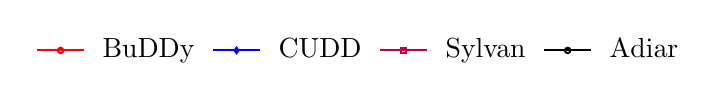
\begin{tikzpicture}
      \begin{customlegend}[
        legend columns=-1,
        legend style={draw=none,column sep=1ex},
        legend entries={BuDDy, CUDD, Sylvan, Adiar}
        ]
        \addlegendimage{style=plot_buddy}
        \addlegendimage{style=plot_cudd}
        \addlegendimage{style=plot_sylvan}
        \addlegendimage{style=plot_adiar}
      \end{customlegend}
    \end{tikzpicture}

    \caption{Minimal running time for the \emph{Queens} problems.}
  \end{figure}
\end{frame}

\begin{frame}
  \frametitle{Adiar v1.2 : Internal Memory}

  \begin{center}
  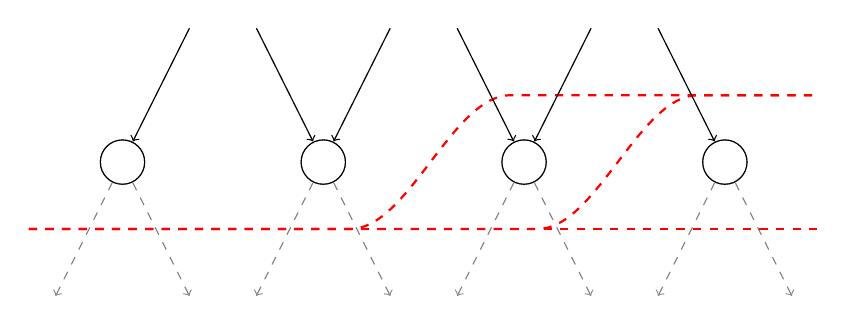
\begin{tikzpicture}[scale=1.7, every node/.style={transform shape}]
    % cut coordinates
    \coordinate (cut_start) at (-0.7,-0.5);
    \coordinate (cut_end_low) at (5.2,-0.5);
    \path (cut_end_low) +(0,1) coordinate (cut_end_high);

    % --------------------------------------------------------------------------
    % before
    \onslide<1> {
      \node[shape = circle, draw = gray] at (0,0)  (0_before) {};
      \draw[gray, dashed, <-] (0_before) -- ++(0.5,1.0);
    }

    % after
    \onslide<2-> {
      \node[shape = circle, draw = black] at (0,0) (0_after) {};
      \draw[black, <-] (0_after) -- ++(0.5,1.0);

      \draw[gray, dashed, ->] (0_after) -- ++(-0.5,-1);
      \draw[gray, dashed, ->] (0_after) -- ++(0.5,-1);
    }

    % --------------------------------------------------------------------------
    % before
    \onslide<-2> {     
      \node[shape = circle, draw = gray] at (1.5,0) (1_before) {};
      \draw[gray, dashed, <-] (1_before) -- ++(-0.5,1.0);
      \draw[gray, dashed, <-] (1_before) -- ++(0.5, 1.0);
    }

    % after
    \onslide<3-> {
      \node[shape = circle, draw = black] at (1.5,0) (1_after) {};
      \draw[black, <-] (1_after) -- ++(-0.5,1.0);
      \draw[black, <-] (1_after) -- ++(0.5, 1.0);

      \draw[gray, dashed, ->] (1_after) -- ++(-0.5,-1);
      \draw[gray, dashed, ->] (1_after) -- ++(0.5,-1);
    }

    % cut
    \onslide<4> {
      \draw[thick, dashed, red]
        (cut_start) -- ++(2.4,0.0) cos ++(0.6,0.5) sin ++(0.6,0.5) -- (cut_end_high)
      ;
    }
    
    % --------------------------------------------------------------------------
    % before
    \onslide<-4> {
      \node[shape = circle, draw = gray] at (3.0,0) (2_before) {};
      \draw[gray, dashed, <-] (2_before) -- ++(-0.5,1.0);
      \draw[gray, dashed, <-] (2_before) -- ++(0.5,1.0);
    }

    % after    
    \onslide<5-> {
      \node[shape = circle, draw = black] at (3.0,0) (2_after) {};
      \draw[black, <-] (2_after) -- ++(-0.5, 1.0);
      \draw[black, <-] (2_after) -- ++(0.5, 1.0);

      \draw[gray, dashed, ->] (2_after) -- ++(-0.5,-1);
      \draw[gray, dashed, ->] (2_after) -- ++(0.5,-1);
    }

    % cut
    \onslide<5> {
      \draw[thick, dashed, red]
        (cut_start) -- ++(3.8,0.0) cos ++(0.6,0.5) sin ++(0.6,0.5) -- (cut_end_high)
      ;
    }

    % --------------------------------------------------------------------------
    % before
    \onslide<-5> {
      \node[shape = circle, draw = gray] at (4.5,0) (3_before) {};
      \draw[gray, dashed, <-] (3_before) -- ++(-0.5,1.0);
    }

    % after
    \onslide<6-> {
      \node[shape = circle, draw = black] at (4.5,0) (3_after) {};
      \draw[black, <-] (3_after) -- ++(-0.5,1.0);      

      \draw[gray, dashed, ->] (3_after) -- ++(-0.5,-1);
      \draw[gray, dashed, ->] (3_after) -- ++(0.5,-1);
    }

    % cut
    \onslide<6> {
      \draw[thick, dashed, red]
        (cut_start) -- (cut_end_low)
      ;
    }
  \end{tikzpicture}
\end{center}
\end{frame}

\begin{frame}
  \frametitle{Adiar v1.2 : Internal Memory}

  \begin{columns}
    \begin{column}{0.55\textwidth}
      \begin{definition}[i-level cut]
        \begin{tikzpicture}[scale=0.9]
          % levels
\node (Lcal) {\color{gray} $\mathcal{L}$};

\node[below=0.5cm of Lcal] (Lj) {\color{gray} $j$};
\node[below=0.5cm of Lj] (Lj1) {\color{gray} $j+1$};
\node[below=0.5cm of Lj1] (Ldots) {\color{gray} $\vdots$};
\node[below=0.6cm of Ldots] (Lji) {\color{gray} $j+i$};

\draw[dashed, gray]
  ($ (Lj) + (1,0) $) edge ($ (Lj) + (7,0) $)
;

\draw[dashed, gray]
  ($ (Lji) + (1,0) $) edge ($ (Lji) + (7,0) $)
;

% nodes
\node[shape = circle, draw = black, fill=white, right=2cm of Lj] (j_1) {};
\node[shape = circle, draw = black, fill=white, right=3cm of Lj] (j_2) {};
\node[shape = circle, draw = black, fill=white, right=5cm of Lj] (j_3) {};

\node[shape = circle, draw = black, fill=white, right=2.5cm of Lj1] (j1_1) {};
\node[shape = circle, draw = black, fill=white, right=4cm of Lj1] (j1_2) {};

\node[right=3.8cm of Ldots] (jdot_1) {$\cdot$};
\node[right=5.3cm of Ldots] (jdot_2) {$\cdot$};

\node[shape = circle, draw = black, fill=white, right=1.5cm of Lji] (ji_1) {};
\node[shape = circle, draw = black, fill=white, right=3cm of Lji] (ji_2) {};
\node[shape = circle, draw = black, fill=white, right=5cm of Lji] (ji_3) {};

% arcs
\draw[->]
% to level j
  ($ (j_1) + (-0.5,0.5) $) edge (j_1)
  ($ (j_1) + (0.5,0.5) $) edge (j_1)

  ($ (j_2) + (0,0.5) $) edge (j_2)

  ($ (j_3) + (-0.5,0.5) $) edge (j_3)
  ($ (j_3) + (0.5,0.5) $) edge (j_3)

% to level j+1
  (j_1) edge (j1_1)
  (j_2) edge (j1_1)
  ($ (j_2) + (1,0.5) $) edge (j1_2)
  (j_3) edge (j1_2)

% to levels in between
  (j1_2) edge[bend right=10] (jdot_1)
  (j1_2) edge[bend left=20] (jdot_2)
  (j_3) edge[bend left=15] (jdot_2)
  (j_3) edge[bend left=50] (jdot_2)

% to level j+i
  ($ (j_1) + (-0.7,0.5) $) edge[bend right=10] (ji_1)
  (j_1) edge[bend left=5] (ji_1)
  (j_2) edge[bend left=5] (ji_2)
  (jdot_1) edge[bend left=10] (ji_2)
  (jdot_2) edge[bend left=20] (ji_3)
  (jdot_2) edge[bend right=20] (ji_3)

% past level j+i
  (j1_1) edge[bend left=5] ($ (ji_1) + (0.7,-0.5) $)
  (jdot_1) edge[bend right=10] ($ (ji_2) + (1,-0.5) $)
  (ji_1) edge ($ (ji_1) + (-0.5,-0.5) $)
  (ji_1) edge ($ (ji_1) + (0.5,-0.5) $)
  (ji_2) edge ($ (ji_2) + (0,-0.5) $)
  (ji_3) edge ($ (ji_3) + (-0.5,-0.5) $)
  ($ (j_3) + (1,0.5) $) -> ($ (ji_3) + (1,-0.5) $)
;

% cut
\draw[thick, dashed, red]
  ($ (j_1) + (-1.2, -1.5) $) sin
  ($ (j_2) + (-0.2, -0.5) $) cos
  ($ (j_2) + (0.4, -2) $) sin
  ($ (jdot_1) + (0.0, -0.5) $) cos
  ($ (jdot_1) + (0.2, 0) $) --
  ($ (j1_2) + (-0.3, 0) $) sin
  ($ (j1_2) + (0, 0.5) $) cos
  ($ (j1_2) + (0.4, 0) $) sin
  ($ (j1_2) + (1.1, -1.8) $) --
  ($ (j1_2) + (2.2, -1.8) $)
;

        \end{tikzpicture}
      \end{definition}
    \end{column}
    \begin{column}{0.44\textwidth}
      \onslide<2-> {
        \begin{lemma}
          The maximum $i$-level cut problem is in P for $i \in \{ 1,2 \}$.
        \end{lemma}
        % \begin{proof}
        %   For each $j$, greedily place each vertice $v$ either in $S$ or in $T$.
        % \end{proof}
      }

      \onslide<3-> {
        \begin{theorem}[\footnotesize Lampis, Kaouri, Mitsou 2011]
          The maximum $i$-level cut problem is NP-complete for $i \geq 4$.
        \end{theorem}
      }
    \end{column}
  \end{columns}
\end{frame}

\begin{frame}
  \frametitle{Adiar v1.2 : Internal Memory}

  \onslide<2-> {
    \begin{theorem}
      The maximum ($i$-level) cut of a BDD with $N$ internal nodes is $N+1$.
    \end{theorem}
    % \begin{proof}
    %   Induction in $N$ for the more general case of a shared decision diagram with
    %   $r$ roots.
    % \end{proof}
  }

  \onslide<3-> {
    \begin{theorem}
      For $i \in \{ 1,2 \}$, the maximum $i$-level cut of the (unreduced) output
      of Apply\\is upper bounded by the product of the inputs' corresponding
      $i$-level cuts.
    \end{theorem}
    % \begin{proof}
    %   Pairing of the input's edges and look at how they relate to the cuts.
    % \end{proof}
  }

  \onslide<4-> {
    \begin{lemma}
      The maximum $2$-level cut of a BDD is upper bounded by $\tfrac{3}{2}$ its
      $1$-level cut.
    \end{lemma}
  }
\end{frame}

% ------------------------------------------------------------------------------
% FUTURE WORK
% ------------------------------------------------------------------------------
\begin{frame}[plain,noframenumbering]{} % \blankframe until reveal
  \begin{figure}
    \centering

    \setvalue{timeline_c0 = gray}
    \setvalue{timeline_c1 = gray}
    \setvalue{timeline_c2 = orange}

    \begin{tikzpicture}
      % Primary line
\draw[thick] (0,0) -- (4,0);
\draw[thick] (4.1,0.2) -- (3.9,-0.2);

\draw[-latex, thick] (4.3,0) -- (12,0);
\draw[thick] (4.4,0.2) -- (4.2,-0.2);

% 1985
\draw (0.1,-0.1) -- ++(0,0.2);
\node at (0.1,-0.3) (y1985) {\tiny $1985$} ;

\draw[dashed, color=\getvalue{timeline_c0}] (0.6,0) -- ++(0,0.8);
\node[color=\getvalue{timeline_c0}, align=left] at (1.4,1.3)
(bryant_1986)
{\footnotesize Bryant (1986)\\Binary Decision Diagram (BDD)};

\draw[dashed, color=\getvalue{timeline_c0}] (0.9,-0) -- ++(0,-0.7);
\node[color=\getvalue{timeline_c0}, align=left] at (0.9,-1.3)
(aggarval_1987)
{\footnotesize Aggarwal \& Vitter (1987)\\I/O-model};

% 1990
\draw (1.8,-0.1) -- ++(0,0.2);
\node at (1.8,-0.3) (y1990) {\tiny $1990$};

% 1995
\draw (3.4,-0.1) -- ++(0,0.2);
\node at (3.4,-0.3) (y1995) {\tiny $1995$};

\draw[dashed, color=\getvalue{timeline_c0}] (3.75,0) -- ++(0,-1.5);
\node[color=\getvalue{timeline_c0}, align=left] at (3.7,-2.1)
(arge_1995)
{\footnotesize Arge (1995)\\BDD + I/O-model};

\draw[dashed, color=\getvalue{timeline_c1}] (4.8,0) -- ++(0,0.8);
\node[color=\getvalue{timeline_c1}, align=left] at (5,1.3)
(v1_0)
{\footnotesize Adiar v1.0\\BDD};

% 2022
\draw (5.8,-0.1) -- ++(0,0.2);
\node at (5.8,-0.3) (y2023)  {\tiny $2022$};

\draw[dashed, color=\getvalue{timeline_c1}] (6.2,0) -- ++(0,-0.8);
\node[color=\getvalue{timeline_c1}, align=left] at (6.2,-1.3)
(v1_1)
{\footnotesize Adiar v1.1\\ZDD};

\draw[dashed, color=\getvalue{timeline_c1}] (7,0) -- ++(0,0.8);
\node[color=\getvalue{timeline_c1}, align=left] at (7.5,1.25)
(v1_2)
{\footnotesize Adiar v1.2\\Internal Memory};

% 2023
\draw (8.5,-0.1) -- ++(0,0.2);
\node at (8.5,-0.3) {\tiny $2023$} (y2023);

\draw[dashed, color=\getvalue{timeline_c2}] (9,0) -- ++(0,-0.8);
\node[color=\getvalue{timeline_c2}, align=left] at (10.3,-1.65)
(v2_0)
{\footnotesize Adiar v2.0\\Multi-variable Quantification\\(Multi-recursion)};

\draw[dashed, color=\getvalue{timeline_c2}] (10.5,0) -- ++(0,0.8);
\node[color=\getvalue{timeline_c2}, align=left] at (10.9,1.25)
(v2_1)
{\footnotesize Adiar v2.1\\Variable Reordering};

% 2024
\draw (11.4,-0.1) -- ++(0,0.2);
\node at (11.4,-0.3) (y2024) {\tiny $2024$};

    \end{tikzpicture}
  \end{figure}
\end{frame}

\begin{frame}
  \frametitle{Adiar v2.0 : Multi-variable Quantification}

  \begin{center}
    \LARGE

    $\mathit{RelProd}(S,T)
    \equiv
    (
    \ {\only<2>{\color{orange}}\exists \vec{x} .}\
    S(\vec{x}) \wedge T(\vec{x}, \vec{x'})
    \ ) [\vec{x'} / \vec{x}]$
  \end{center}
\end{frame}

\begin{frame}[fragile]
  \frametitle{Adiar v2.0 : Multi-variable Quantification}

  \begin{figure}
    \centering

    \begin{lstlisting}[language=sml]
*@{\bf exists}@*($f$, $V$)
  if $f = \bot \lor f = \top$
       then $f$
  else if $V \cap \{ i \in \N \mid i \geq \texttt{top}(f) \} = \emptyset$
       then $f$
  else if top($f$) $\not\in V$
       then Node { top($f$), *@{\bf exists}@*($f$.low, $V$), *@{\bf exists}@*($f$.high, $V$) }
  else let low  = *@{\bf exists}@*($f$.low, $V$)
           high = *@{\bf exists}@*($f$.high, $V$)
       in *@{\bf or}@*(low, high)
    \end{lstlisting}
  \caption{A recursive multi-variable {\bf exists} operation.}
\end{figure}

  \begin{tikzpicture}[overlay]
    \onslide<2-> {
      \draw[draw=none, fill=white, fill opacity=0.7] (0.2,4.3) rectangle ++(13.5,2);
    }

    \onslide<1,3-> {
      \draw[draw=none, fill=white, fill opacity=0.7] (0.2,3.3) rectangle ++(13.5,1);
    }

    \onslide<-2> {
      \draw[draw=none, fill=white, fill opacity=0.7] (0.2,1.9) rectangle ++(13.5,1.4);
    }
  \end{tikzpicture}

\end{frame}

\begin{frame}
  \frametitle{Adiar v2.0 : Multi-variable Quantification}

  \begin{center}
  \begin{tikzpicture}
    % Sweepline
    \onslide<2> { \draw[gray, thick, dashed] (-2.5, -5.0) -- (10, -5.0); }
    \onslide<3> { \draw[gray, thick, dashed] (-2.5, -4.2) -- (10, -4.2); }
    \onslide<4-9> { \draw[gray, thick, dashed] (-2.5, -3.2) -- (10, -3.2); }

    \onslide<4>   { \draw[gray, thick, dashed] (2.5, -3.4) -- (9.7, -3.4); }
    \onslide<5,9> { \draw[gray, thick, dashed] (2.5, -4.2) -- (9.7, -4.2); }
    \onslide<6-8> { \draw[gray, thick, dashed] (2.5, -5.0) -- (9.7, -5.0); }

    \onslide<10> { \draw[gray, thick, dashed] (-2.5, -2.5) -- (10, -2.5); }
    \onslide<11> { \draw[gray, thick, dashed] (-2.5, -1.7) -- (10, -1.7); }
    \onslide<12> { \draw[gray, thick, dashed] (-2.5, 0) -- (10, 0); }

    % --------------------------------------------------------------------------
    % INPUT
    \draw[blue, thick] (-1.8,-5.0) -- (-2.0,-4.2) -- (-1.4,-1.7) -- (-0.1,0.1)
                    -- (0.1,0.1)  -- (1.4,-1.7)  -- (2.0,-4.2)  -- (1.8,-5.0);

    \draw[red, thick] (-1.8,-5.0) -- (-1.6,-5.6)
                      (1.8,-5.0) -- (1.6,-5.6);

    \onslide<11-> {
      \node[shape = circle, draw = black, fill = white]
      (i_root) {};
    }

    \onslide<10-> {
      \node[shape = circle, draw = black, fill = white,
            below right=1.4cm and 0.2cm of i_root]
      (i_p1) {};
    }

    \onslide<11-> {
      \draw[->, blue] (i_p1) edge (i_root);
    }

    \onslide<3-> {
      \node[shape = circle, draw = black, fill = white,
            below left=0.55cm and 0.2cm of i_p1]
      (i_p2) {};
    }

    \onslide<10-> {
      \draw[->, dashed, blue] (i_p2) edge (i_p1);
    }

    \onslide<3-> {
      \node[shape = circle, draw = black, fill = white,
            below right=0.5cm and 0.2cm of i_p2]
      (i_quant2) {\tiny $x_j$};
    }

    \onslide<4-> {
      \draw[->, blue, thick] (i_quant2) edge (i_p2);
    }

    \onslide<2-> {
      \node[shape = circle, draw = black, fill = white,
            below left=0.55cm and 0.2cm of i_quant2]
      (i_p3_1) {};

      \node[shape = circle, draw = black, fill = white,
            below right=0.55cm and 0.2cm of i_quant2]
      (i_p3_2) {};
    }

    \onslide<3-> {
      \draw[->, blue, thick, dashed] (i_p3_1) edge (i_p2);
      \draw[->, blue, dashed] (i_p3_1) edge (i_quant2);
      \draw[->, blue] (i_p3_2) edge (i_quant2);
    }

    \onslide<2-> {
      \node[shape = circle, draw = black, fill = white,
            below left=0.55cm and 0.2cm of i_p3_1]
      (i_p4_1) {};

      \node[shape = circle, draw = black, fill = white,
            below left=0.55cm and 0.2cm of i_p3_2]
      (i_p4_2) {};

      \draw[->, blue, dashed]
        (i_p4_1) edge (i_p3_1)
        (i_p4_2) edge (i_p3_2)
      ;
    }

    \node[shape = rectangle, draw = red, fill = white,
      below right=5.4cm and -0.3cm of i_root]
    (i_p5_1) {};

    \node[shape = rectangle, draw = red, fill = white,
      below right=5.4cm and 0.7cm of i_root]
    (i_p5_2) {};

    \onslide<2-> {
      \draw[->, red]
        (i_p4_1) edge (i_p5_1)
        (i_p4_2) edge (i_p5_2)
      ;
    }

    % --------------------------------------------------------------------------
    % REDUCED OUTPUT
    \onslide<2-6,8-> {
      \draw[thick] (3.0,-5.0) -- (3.2,-5.6)
                   (5.3,-5.0) -- (5.1,-5.6)
      ;
          
      \node[shape = rectangle, draw = black, fill = white,
            right=3.5cm of i_p5_1]
      (o1_p5_1) {};

      \node[shape = rectangle, draw = black, fill = white,
            right=3.5cm of i_p5_2]
      (o1_p5_2) {};

      \node[shape = circle, draw = black, fill = white,
            right=3.5cm of i_p4_1]
      (o1_p4_1) {};

      \node[shape = circle, draw = black, fill = white,
            right=3.5cm of i_p4_2]
      (o1_p4_2) {};

      \draw[->]
        (o1_p4_1) edge (o1_p5_1)
        (o1_p4_2) edge (o1_p5_2)
      ;
    }

    \onslide<3-5,9-> {
      \draw[thick] (2.9,-4.2) -- (3.0,-5.0)
                   (5.5,-4.2) -- (5.3,-5.0)
      ;

      \node[shape = circle, draw = black, fill = white,
            right=3.5cm of i_p3_1]
      (o1_p3_1) {};

      \node[shape = circle, draw = black, fill = white,
            right=3.5cm of i_p3_2]
      (o1_p3_2) {};

      \draw[->, dashed]
        (o1_p3_1) edge (o1_p4_1)
        (o1_p3_2) edge (o1_p4_2)
      ;
    }

    \onslide<4> {
      \draw[thick, dotted] (3.2,-3.4) -- (2.9,-4.2)
                           (5.1,-3.4) -- (5.5,-4.2)
      ;
    }

    \onslide<10-> {
      \draw[thick] (2.8,-2.5) -- (2.9,-4.2)
                   (4.8,-2.5) -- (5.5,-4.2)
      ;

      \node[shape = circle, draw = black, fill = white,
            right=3.5cm of i_p2]
      (o1_p2) {};

      \draw[->, dashed] (o1_p2) edge (o1_p3_1);
      \draw[->] (o1_p2) edge (o1_p3_2);
    }

    \onslide<11-> {
      \draw[thick] (2.9,-1.7) -- (2.8,-2.5)
                   (4.6,-1.7) -- (4.8,-2.5)
      ;

      \node[shape = circle, draw = black, fill = white,
            right=3.5cm of i_p1]
      (o1_p1) {};

      \draw[->, dashed] (o1_p1) edge (o1_p2);
    }

    \onslide<12-13> {
      \draw[thick] (3.8,0) -- (2.9,-1.7)
                   (4.0,0) -- (4.6,-1.7)
      ;

      \node[shape = circle, draw = black, fill = white,
            right=3.5cm of i_root]
      (o1_root) {};

      \draw[->] (o1_root) edge (o1_p1);
    }

    % --------------------------------------------------------------------------
    % SECOND SWEEP
    \onslide<5-9> {
      \draw[blue, thick, dotted] (6.95, -2.9) -- (6.9,-3.2)
                                 (9.15, -2.9) -- (9.2,-3.2)
          ;

      \draw[blue, thick] (6.9,-3.2) -- (6.8, -4.2)
                         (9.2,-3.2) -- (9.4, -4.2)
      ;
          
      \node[shape = circle, draw = none, % dummy for crossing in-going arcs
            right=3.5cm of o1_p2]
      (o2_p2) {};

      \node[shape = circle, draw = black, fill = white,
            right=3.5cm of o1_p3_1]
      (o2_p3_1) {};

      \node[shape = circle, draw = black, fill = white,
            right=3.5cm of o1_p3_2]
      (o2_p3_2) {};

      \draw[->, thick, blue, dashed] (o2_p3_1) edge (o2_p2);
      \draw[->, thick, blue] (o2_p3_2) edge (o2_p2);
    }

    \onslide<6-8> {
      \draw[blue, thick] (6.8, -4.2) -- (6.9, -5.0)
                         (9.4, -4.2) -- (9.3, -5.0)
      ;

      \node[shape = circle, draw = black, fill = white,
            right=3.5cm of o1_p4_1]
      (o2_p4_1) {};

      \node[shape = circle, draw = black, fill = white,
            right=3.5cm of o1_p4_2]
      (o2_p4_2) {};

      \draw[->, blue, dashed]
        (o2_p4_1) edge (o2_p3_1)
        (o2_p4_2) edge (o2_p3_2)
      ;

      \draw[red, thick] (6.9, -5.0) -- (7.2, -5.6)
                        (9.3, -5.0) -- (9.0, -5.6)
      ;

      \node[shape = rectangle, draw = red, fill = white,
            right=3.5cm of o1_p5_1]
      (o2_p5_1) {};

      \node[shape = rectangle, draw = red, fill = white,
            right=3.5cm of o1_p5_2]
      (o2_p5_2) {};

      \draw[->, red]
        (o2_p4_1) edge (o2_p5_1)
        (o2_p4_2) edge (o2_p5_2)
      ;
    }
  \end{tikzpicture}
\end{center}
\end{frame}

\blankframe

\begin{frame}
  \frametitle{Adiar v2.1 : Variable Reordering}

  \begin{center}
    \LARGE

    $\mathit{RelProd}(S,T)
    \equiv
    (
    \ {\color{orange}}\exists \vec{x} .\
    S(\vec{x}) \wedge T(\vec{x}, \vec{x'})
    \ ) {\color{orange} [\vec{x'} / \vec{x}]}$
  \end{center}
\end{frame}

\begin{frame}[fragile]
  \frametitle{Adiar v2.1 : Variable Reordering}

  \begin{columns}
    \begin{column}{0.45\textwidth}
      \begin{figure}
        \centering

        \begin{lstlisting}[language=sml]
*@{\bf substitute}@*($f$, $i\_map$)
  let low  = *@{\bf substitute}@*($f$.low)
      high = *@{\bf substitute}@*($f$.high)
      i'   = $i\_map$[top($f$)]
  in *@{\bf bubble}@*(i', low, high)
        \end{lstlisting}

        \begin{tikzpicture}[overlay]
          \onslide<1,3-8> {
            \draw[draw=none, fill=white, fill opacity=0.7] (-2.8,1.5) rectangle ++(6,1);
          }

          \onslide<-2,4-8> {
            \draw[draw=none, fill=white, fill opacity=0.7] (-2.8,1) rectangle ++(6,0.6);
          }

          \onslide<-3> {
            \draw[draw=none, fill=white, fill opacity=0.7] (-2.8,0.5) rectangle ++(6,0.6);
          }
        \end{tikzpicture}

        \caption{A recursive {\bf substitute} operation.}
      \end{figure}
    \end{column}
    \begin{column}{0.55\textwidth}
      \only<1-8>{
        \begin{figure}
          \centering

          {\footnotesize $[ 0 \mapsto 3, 1 \mapsto 0, 2 \mapsto 2, 3 \mapsto 1 ]$}

          \vspace{5pt}

          \begin{tikzpicture}
            % ------------------------------------------------------------------
            % leaves
            \node[shape = rectangle, draw = black] at (1,-4)
            (sink_F) {$\bot$};

            \node[shape = rectangle, draw = black] at (-1,-4)
            (sink_T) {$\top$};

            % ------------------------------------------------------------------
            % state: start
            \onslide<1-4>{
              \node[shape = circle, draw = black]
              (0) {$x_0$};
            }

            \onslide<1>{
              \node[shape = circle, draw = black, below left=1.4cm and .5cm of 0]
              (21) {$x_2$};

              \node[shape = circle, draw = black, below right=1.4cm and .5cm of 0]
              (22) {$x_2$};

              \node[shape = circle, draw = black, below right=0.4cm and .5cm of 21]
              (3) {$x_3$};

              \draw[->, dashed]
                (0)  edge (21)
                (21) edge (sink_T)
                (22) edge (3)
                (3)  edge (sink_T)
              ;

              \draw[->]
                (0)  edge (22)
                (21) edge (3)
                (22) edge (sink_F)
                (3)  edge (sink_F)
              ;
            }

            % ------------------------------------------------------------------
            % state: recursively sorted + bubble before
            \onslide<2-5>{
              \node[shape = circle, draw = black, below left=0.4cm and .5cm of 0]
              (11) {$x_1$};

              \node[shape = circle, draw = black, below right=0.4cm and .5cm of 0]
              (12) {$x_1$};
            }

            \onslide<2-6>{
              \node[shape = circle, draw = black, below right=0.4cm and .5cm of 11]
              (2) {$x_2$};
            }

            \onslide<2-4>{
              \draw[->, dashed] (0)  edge (11);
              \draw[->] (0)  edge (12);
            }

            \onslide<2-5> {
              \draw[->, dashed]
                (11) edge (sink_T)
                (12) edge (2)
              ;

              \draw[->]
                (11) edge (2)
                (12) edge (sink_F)
              ;
            }

            \onslide<2-6> {
              \draw[->, dashed] (2) edge (sink_T);
              \draw[->] (2)  edge (sink_F);
            }

            % ------------------------------------------------------------------
            % state: bubble after
            \onslide<6->{
              \node[shape = circle, draw = black, below=.2cm of 0]
              (bubble_1) {$x_1$};
            }

            \onslide<7->{
              \node[shape = circle, draw = black, below left=0.4cm and .5cm of bubble_1]
              (bubble_21) {$x_2$};
              \node[shape = circle, draw = black, below right=0.4cm and .5cm of bubble_1]
              (bubble_22) {$x_2$};

              \draw[->, dashed]
                (bubble_1) edge (bubble_21)
                (bubble_21) edge (sink_T)
              ;

              \draw[->]
                (bubble_1) edge (bubble_22)
                (bubble_22) edge (sink_F)
              ;
            }

            \onslide<8->{
              \node[shape = circle, draw = black, below right=0.4cm and .5cm of bubble_21]
              (bubble_3) {$x_3$};

              \draw[->, dashed]
                (bubble_22) edge (bubble_3)
                (bubble_3) edge (sink_T)
              ;

              \draw[->]
                (bubble_21) edge (bubble_3)
                (bubble_3) edge (sink_F)
              ;
            }
          \end{tikzpicture}

          \caption{%
            \only<1>{$\neg (x_0 \ ?\ x_2 \vee x_3 \ :\ x_2 \wedge x_3)$}%
            \only<2-4>{$\neg (x_0 \ ?\ x_2 \vee x_1 \ :\ x_2 \wedge x_1)$}%
            \only<5-7>{$\dots$}%
            \only<8->{$\neg (x_3 \ ?\ x_2 \vee x_1 \ :\ x_2 \wedge x_1)$}%
          }
        \end{figure}
      }
      \only<9->{
        \begin{table}
          \centering

          \begin{tabular}{c c c}
            Time    & Space   & I/O
            \\ \hline
            $O(NT)$ & $O(NT)$ & $O(NT)$
          \end{tabular}

          \caption{Complexity of depth-first {\bf substitute}}
        \end{table}

        \onslide<10->{
          \begin{table}
            \centering

            \begin{tabular}{c c c}
              Time    & Space   & I/O
              \\ \hline
              $O(N T \log T)$ & $O(N+T)$ & $O(N \cdot \sort(T))$
            \end{tabular}

            \caption{Complexity of level-by-level {\bf substitute}}
          \end{table}
        }
      }
    \end{column}
  \end{columns}
\end{frame}

\begin{frame}
  \frametitle{Adiar v2.1 : Variable Reordering}

  \begin{problem}[Variable Replacement]
    Given BDD $f_{\pi}$ with variable ordering $\pi$ and remapping of variables
    $m : \N \rightarrow \N$,\\
    construct $f'_{\pi} \equiv f_{\pi}[x / m(x)]$.
  \end{problem}

  \pause

  \begin{problem}[Static Variable Reordering]
    Given BDD $f_{\pi}$ with variable ordering $\pi$ and another variable
    ordering $\pi'$,\\
    construct $f_{\pi'} \equiv f_{\pi}$.
  \end{problem}

  \pause

  \begin{problem}[Dynamic Variable Reordering]
    Given BDD $f_{\pi}$ with variable ordering $\pi$,\\
    find $\pi'$ and construct $f_{\pi'} \equiv f_{\pi}$ such that
    $\abs{f_{\pi'}}$ is minimal.
  \end{problem}
\end{frame}

% ------------------------------------------------------------------------------
% END
% ------------------------------------------------------------------------------
\blankframe

\begin{frame}[plain,noframenumbering]{} % \blankframe until reveal
  \begin{figure}
    \centering

    \setvalue{timeline_c0 = gray}
    \setvalue{timeline_c1 = black}
    \setvalue{timeline_c2 = black}

    \begin{tikzpicture}
      % Primary line
\draw[thick] (0,0) -- (4,0);
\draw[thick] (4.1,0.2) -- (3.9,-0.2);

\draw[-latex, thick] (4.3,0) -- (12,0);
\draw[thick] (4.4,0.2) -- (4.2,-0.2);

% 1985
\draw (0.1,-0.1) -- ++(0,0.2);
\node at (0.1,-0.3) (y1985) {\tiny $1985$} ;

\draw[dashed, color=\getvalue{timeline_c0}] (0.6,0) -- ++(0,0.8);
\node[color=\getvalue{timeline_c0}, align=left] at (1.4,1.3)
(bryant_1986)
{\footnotesize Bryant (1986)\\Binary Decision Diagram (BDD)};

\draw[dashed, color=\getvalue{timeline_c0}] (0.9,-0) -- ++(0,-0.7);
\node[color=\getvalue{timeline_c0}, align=left] at (0.9,-1.3)
(aggarval_1987)
{\footnotesize Aggarwal \& Vitter (1987)\\I/O-model};

% 1990
\draw (1.8,-0.1) -- ++(0,0.2);
\node at (1.8,-0.3) (y1990) {\tiny $1990$};

% 1995
\draw (3.4,-0.1) -- ++(0,0.2);
\node at (3.4,-0.3) (y1995) {\tiny $1995$};

\draw[dashed, color=\getvalue{timeline_c0}] (3.75,0) -- ++(0,-1.5);
\node[color=\getvalue{timeline_c0}, align=left] at (3.7,-2.1)
(arge_1995)
{\footnotesize Arge (1995)\\BDD + I/O-model};

\draw[dashed, color=\getvalue{timeline_c1}] (4.8,0) -- ++(0,0.8);
\node[color=\getvalue{timeline_c1}, align=left] at (5,1.3)
(v1_0)
{\footnotesize Adiar v1.0\\BDD};

% 2022
\draw (5.8,-0.1) -- ++(0,0.2);
\node at (5.8,-0.3) (y2023)  {\tiny $2022$};

\draw[dashed, color=\getvalue{timeline_c1}] (6.2,0) -- ++(0,-0.8);
\node[color=\getvalue{timeline_c1}, align=left] at (6.2,-1.3)
(v1_1)
{\footnotesize Adiar v1.1\\ZDD};

\draw[dashed, color=\getvalue{timeline_c1}] (7,0) -- ++(0,0.8);
\node[color=\getvalue{timeline_c1}, align=left] at (7.5,1.25)
(v1_2)
{\footnotesize Adiar v1.2\\Internal Memory};

% 2023
\draw (8.5,-0.1) -- ++(0,0.2);
\node at (8.5,-0.3) {\tiny $2023$} (y2023);

\draw[dashed, color=\getvalue{timeline_c2}] (9,0) -- ++(0,-0.8);
\node[color=\getvalue{timeline_c2}, align=left] at (10.3,-1.65)
(v2_0)
{\footnotesize Adiar v2.0\\Multi-variable Quantification\\(Multi-recursion)};

\draw[dashed, color=\getvalue{timeline_c2}] (10.5,0) -- ++(0,0.8);
\node[color=\getvalue{timeline_c2}, align=left] at (10.9,1.25)
(v2_1)
{\footnotesize Adiar v2.1\\Variable Reordering};

% 2024
\draw (11.4,-0.1) -- ++(0,0.2);
\node at (11.4,-0.3) (y2024) {\tiny $2024$};

    \end{tikzpicture}
  \end{figure}
\end{frame}

\end{document}